\begin{frame}
  \frametitle{Contexte (2)}
  \visible<1->{
    \only<1>{
      \begin{center}
        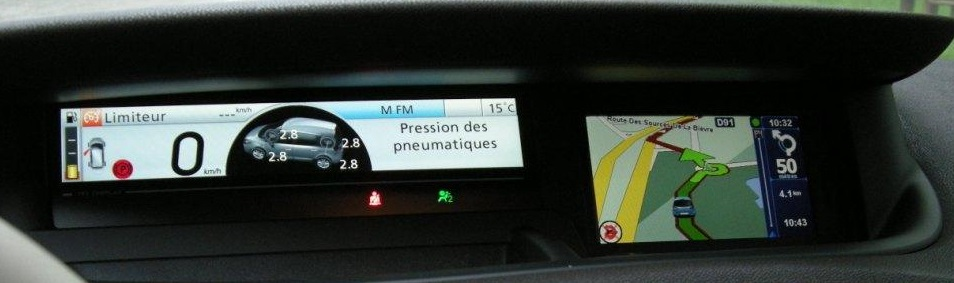
\includegraphics[scale=0.7]{include/tableau_de_bord1.jpg}
      \end{center}
    }
    \only<2->{
      \begin{center}
        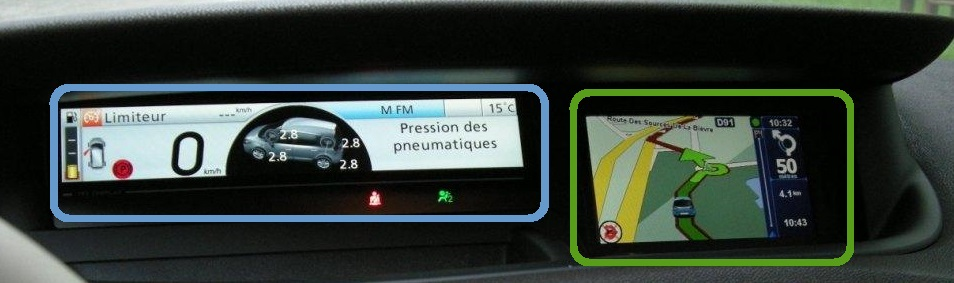
\includegraphics[scale=0.7]{include/tableau_de_bord2.jpg}
      \end{center}
    }
  }
  \visible<3->{
    \begin{center}
      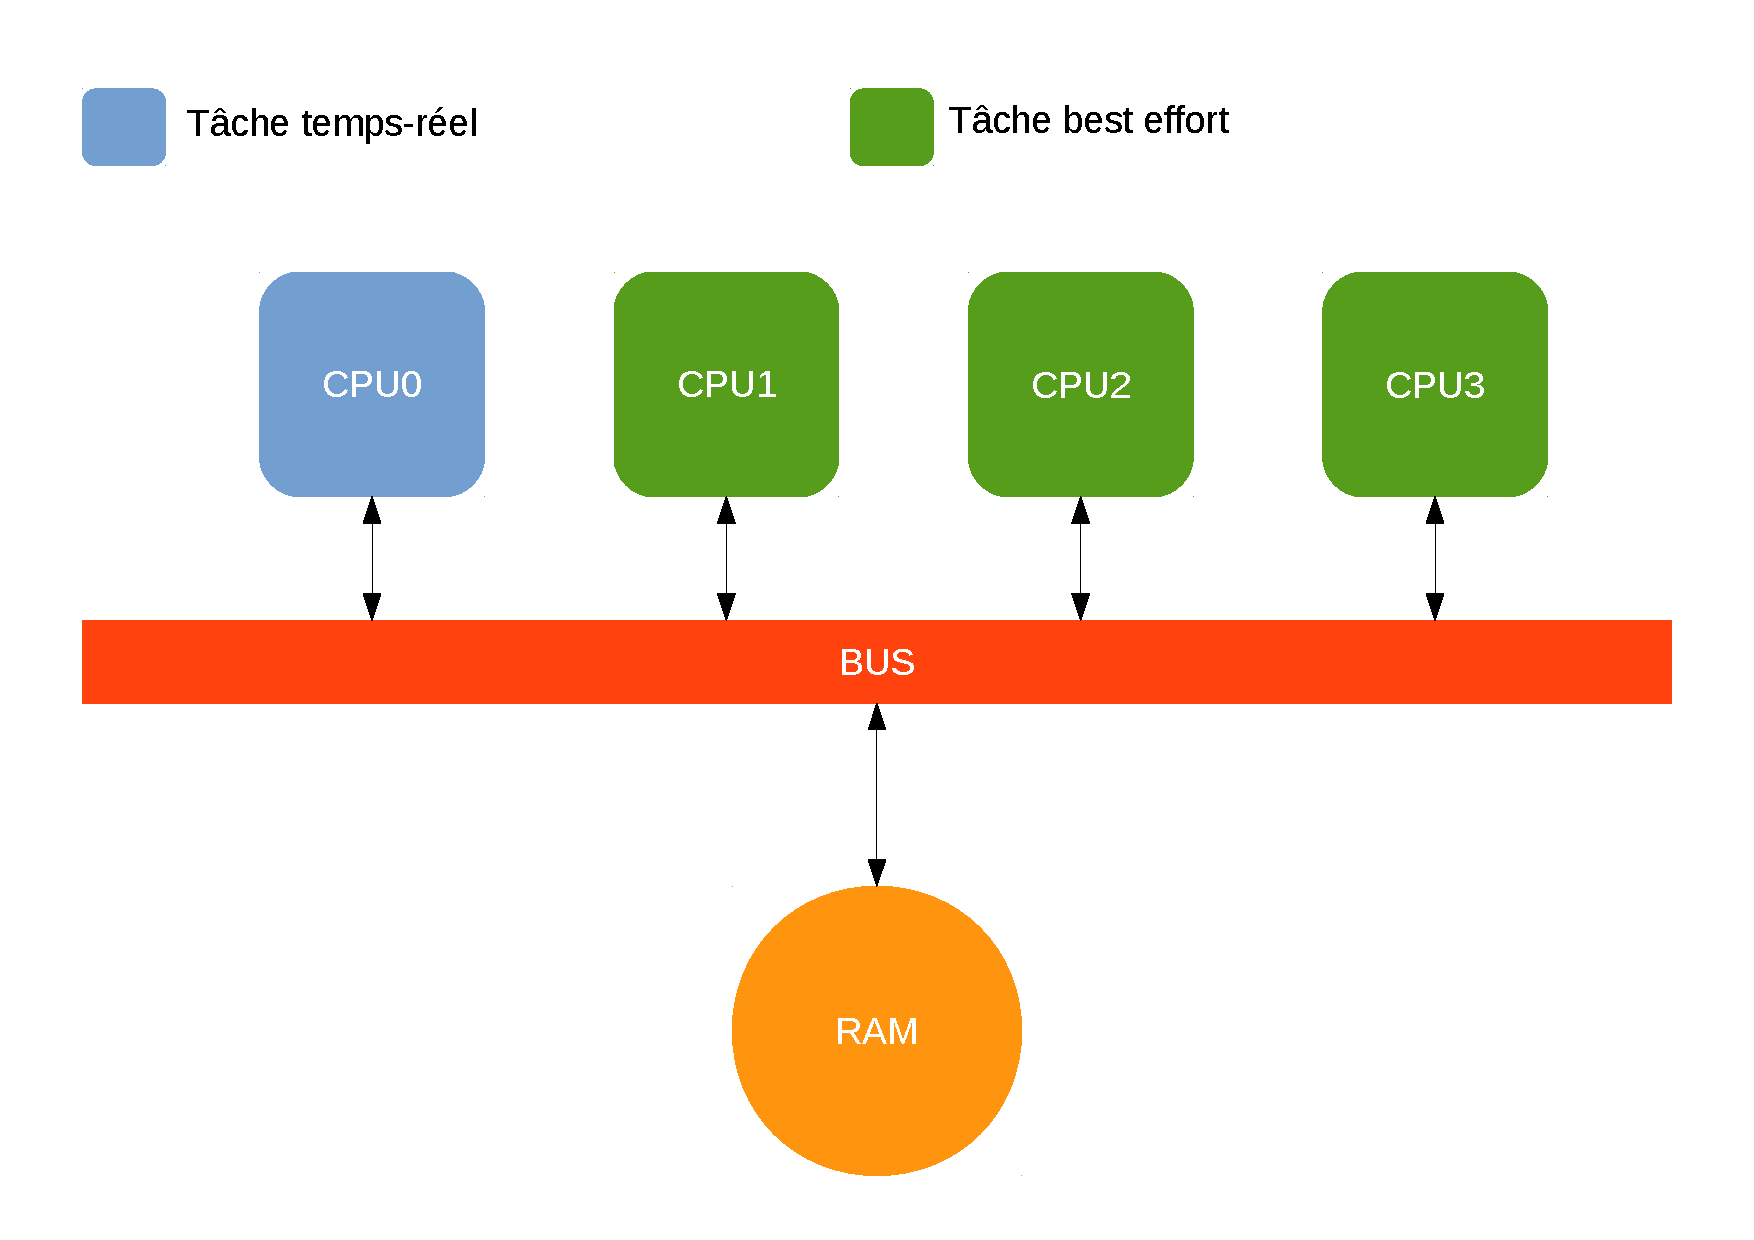
\includegraphics[trim=0 0 0 130,clip,scale=0.2]{include/archi.pdf}
    \end{center}
  }
  \visible<4>{
    \begin{alertblock}{Problèmes}
      Gestion du partage des ressources, et notamment du bus.
    \end{alertblock}
  }
\end{frame}

\begin{frame}
  \frametitle{Objectifs}
  Placé dans le cadre de la thèse d'Antoine Blin en cours au Lip6, ce projet SAR
  a pour objectifs :
  \vspace{1em}
  \begin{enumerate}
  \item Le choix d'une application pour automobile à fort trafic mémoire
    \vspace{1em}
  \item Le portage de cette application sur la carte embarquée
    \vspace{1em}
  \item La parallélisation de cette application
    \vspace{1em}
  \item L'étude de l'impact de cette application sur une tâche temps-réel
  \end{enumerate}
\end{frame}

\begin{frame}
  \frametitle{Choix de l'application}
  \framesubtitle{Critères de sélection}
  \begin{block}{Type d'application}
    Nous avons choisi de porter une application de calcul d'itinéraires car elles
    manipulent des graphes de tailles importantes.
  \end{block}
  Les autres critères sont :
  \begin{itemize}
  \item Langage : pas de \textit{JVM}
    \vspace{1em}
  \item Consommation mémoire contenue : 1 Go de RAM sur la carte
    \vspace{1em}
  \item Nombre de dépendances faible
    \vspace{1em}
  \item Parallélisable
  \end{itemize}
\end{frame}

\begin{frame}
  \frametitle{Choix de l'application}
  \framesubtitle{Comparaison des candidats}
  \begin{block}{}
    Deux applications, écrites en C++ et C, se sont dégagées :
  \end{block}
  \begin{tabular}{c|c}
    \textbf{Open Street Routing Machine} & \textbf{Routino} \\
    \hline
    \visible<2->{
      \begin{minipage}{5cm}
        \vspace{1em}
        \begin{itemize}
        \item[$+$] Parallèle (client-serveur)
          \vspace{1em}
        \item[$-$] Nombre de dépendances
          \vspace{1em}
        \item[$-$] Trop gourmand en mémoire
        \end{itemize}
      \end{minipage}
    }
    &
    \visible<3->{
      \begin{minipage}{5cm}
        \vspace{1em}
        \begin{itemize}
        \item[$+$] Aucune dépendance
          \vspace{1em}
        \item[$+$] Peu gourmand en mémoire
          \vspace{1em}
        \item[$-$] Pas parallèle
        \end{itemize}
      \end{minipage}
    }
  \end{tabular}
  \visible<4->{
    \begin{exampleblock}{Application choisie}
      Routino pour sa facilité de portage et son occupation mémoire contenue.
    \end{exampleblock}
  }
\end{frame}

